\documentclass[conference]{IEEEtran}
\IEEEoverridecommandlockouts

\usepackage{cite}
\usepackage{amsmath,amssymb,amsfonts}
\usepackage{algorithmic}
\usepackage{graphicx}
\usepackage{textcomp}
\usepackage{xcolor}
\usepackage{booktabs}
\usepackage{multirow}
\usepackage{url}
\usepackage{hyperref}
\usepackage{placeins}

\renewcommand{\dbltopfraction}{0.95}
\renewcommand{\dblfloatpagefraction}{0.95}

\graphicspath{{figures/}}

\def\BibTeX{{\rm B\kern-.05em{\sc i\kern-.025em b}\kern-.08em
    T\kern-.1667em\lower.7ex\hbox{E}\kern-.125emX}}

\begin{document}

\title{Lexically Constrained and Interpretable Decoding for Neural Machine Translation}

\author{
\IEEEauthorblockN{Alkım Gönenç Efe}
\IEEEauthorblockA{\textit{Department of Computer Engineering} \\
\textit{İzmir Katip Çelebi University}\\
İzmir, Turkey}
}

\maketitle

\begin{abstract}
Lexically constrained decoding allows users to inject domain-specific terminology into Neural Machine Translation (NMT) output at inference time, without retraining. While prior work has mostly followed structural approaches such as Grid Beam Search and Dynamic Beam Allocation, this paper takes a different route: adjusting raw output logits at each decoding step within a standard beam search pipeline. We implement and evaluate six strategies for English-to-Turkish (EN→TR) and Turkish-to-English (TR→EN) translation---hard exclusion, hard inclusion with dynamic anchor scheduling, soft penalty, curriculum-anchored soft reward with escalation, and two combined modes---using the Helsinki-NLP OPUS-MT models on a bilingual test set of 500 sentence pairs per direction. Hyperparameters are optimized separately per direction using Optuna. Soft reward with escalation achieves the best quality-satisfaction trade-off in both directions: 99.2\%/98.8\% satisfaction with Baseline BLEU of 72.32/81.65 and a near-natural length ratio of 1.062/1.058. Hard inclusion reaches 99.6\%/99.2\% satisfaction while running 2.1--3.3$\times$ faster than the HuggingFace Dynamic Beam Allocation (DBA) baseline. DBA's structural beam allocator exhibits severe length inflation in EN→TR (length ratio 2.768), a direct consequence of agglutinative Turkish morphology forcing it to append words rather than place them inline. In TR→EN the same issue is far milder (1.289). We also report the \emph{logit squeeze effect} in combined modes, the threshold suppression phenomenon in soft penalty, and the challenges of exact-match enforcement in agglutinative Turkish.
\end{abstract}

\begin{IEEEkeywords}
neural machine translation, lexical constraints, constrained decoding, logit manipulation, beam search, Turkish NLP, hyperparameter optimization
\end{IEEEkeywords}

% =============================================================================
\section{Introduction}
% =============================================================================

Transformer-based neural machine translation (NMT) \cite{vaswani2017attention} produces fluent translations, but practical systems often require domain-specific terminology that the model would not otherwise generate. A medical system must use the approved drug name; a legal translation must match jurisdiction-specific terms. Retraining for each domain is expensive, and fine-tuning risks catastrophic forgetting.

Lexically constrained decoding addresses this by enforcing vocabulary constraints at inference time, without modifying model weights. Hokamp and Liu \cite{hokamp2017lexically} introduced Grid Beam Search (GBS), which tracks constraint satisfaction across the beam. Post and Vilar \cite{post2018fast} improved efficiency with Dynamic Beam Allocation (DBA), and Hu et al.~\cite{hu2019improved} extended GBS to phrasal constraints. NeuroLogic Decoding \cite{lu2021neurologic} encodes constraints as logical predicates over the generation space.

Rather than altering the beam search structure, we explore \emph{logit-level} enforcement: directly adjusting raw output logits at each step within the standard HuggingFace Transformers pipeline \cite{wolf2020transformers}. The approach requires no changes to beam search internals and plugs into any model that exposes a LogitsProcessor interface.

We implement six decoding strategies---hard exclusion, hard inclusion with dynamic anchor scheduling, soft penalty, soft curriculum reward with escalation, and two combined modes---and evaluate them on a bilingual set of 500 EN$\leftrightarrow$TR sentence pairs per direction, split into HPO and held-out evaluation sets. Optuna \cite{akiba2019optuna} is used to optimize the logit pressure settings for each translation direction. We benchmark these methods against the HuggingFace DBA implementation under a morphology-aware configuration that provides it with full suffix and capitalization disjunctions. During evaluation we observed several practical issues, including the \emph{logit squeeze} phenomenon in combined modes, threshold suppression in soft penalty, and exact-match failures in Turkish morphology.

% =============================================================================
\section{Related Work}
% =============================================================================

\subsection{Constrained Machine Translation}

Existing constrained decoding methods fall into three categories: structural beam-search modifications, training-time terminology integration, and decoding-time control. Structural methods such as Grid Beam Search (GBS) \cite{hokamp2017lexically} and Dynamic Beam Allocation (DBA) \cite{post2018fast} modify the search algorithm to explicitly track constraint satisfaction states, guaranteeing terminology inclusion at the cost of execution complexity or beam allocation overhead. Phrasal variants \cite{hu2019improved} extend this coverage to multi-token spans. In contrast, terminology-aware training \cite{dinu2019training} bakes terminology tags directly into model parameters, teaching the network to align source terminology tags with target words. While training-time methods avoid decoding-time overhead, they cannot adapt dynamically to unseen terminology at inference time without retraining or fine-tuning.

\subsection{Logit Manipulation and Decoding Control}

Our approach operates entirely through logit manipulation during decoding. Modifying raw logits has been used to guide vocabulary selection in image captioning \cite{anderson2017guided}, steer search trajectories via gradient signals \cite{sha2020gradient}, or prevent generation degeneracy \cite{holtzman2020curious}. In free-text generation, methods like NeuroLogic decoding \cite{lu2021neurologic} resolve lexical constraints as logical predicates over candidates, and sample-based generators \cite{miao2019cgmh} utilize Metropolis-Hastings steps. Unlike these methods, which require scoring completed sequences or altering standard beam states, our logit processors inject pressure directly at each decoding step. Furthermore, they address the subword segmentation and inflection boundaries typical of agglutinative translation.

\subsection{Morphological Alignment and Tuning}

Agglutinative target languages like Turkish present significant alignment challenges for subword tokenization schemes (e.g., BPE \cite{sennrich2016bpe}) used in modern NMT models \cite{tiedemann2020opus}. Suffix chains and phonetic variations mean a target lemma often mismatches the required exact-match surface constraints. While automated hyperparameter optimization is widely used to calibrate neural networks \cite{akiba2019optuna}, we apply it here to balance the logit-level boundaries, escalation thresholds, and morphological penalties necessary to translate morphologically rich targets.


% =============================================================================
\section{Methodology}
% =============================================================================

\subsection{System Architecture}

We use the Helsinki-NLP OPUS-MT English--Turkish models \cite{tiedemann2020opus, tiedemann2023democratizing} implemented in Hugging Face Transformers \cite{wolf2020transformers}. Decoding uses 16-beam search \cite{freitag2017beam} (maximum length 128, no-repeat 3-gram), with constraints applied through the LogitsProcessor interface before beam selection. The implementation is written in PyTorch \cite{paszke2019pytorch}.

An important preprocessing step is token expansion: each constraint word is tokenized into all plausible surface-form variants (capitalized, lowercase, with leading space, etc.). For Turkish inclusion constraints, we also enumerate common morphological suffixes to build a set of acceptable token sequences. Unlike English, where target words usually map one-to-one with surface forms, Turkish routinely concatenates grammatical roles directly onto the noun root. If the model is constrained to output the bare root but the context demands an accusative or dative suffix, exact-match enforcement will fail and force the word into unnatural syntactic positions. This expansion step partially addresses the agglutination mismatch discussed in Section~II-C.

\begin{figure*}[!t]
\centering
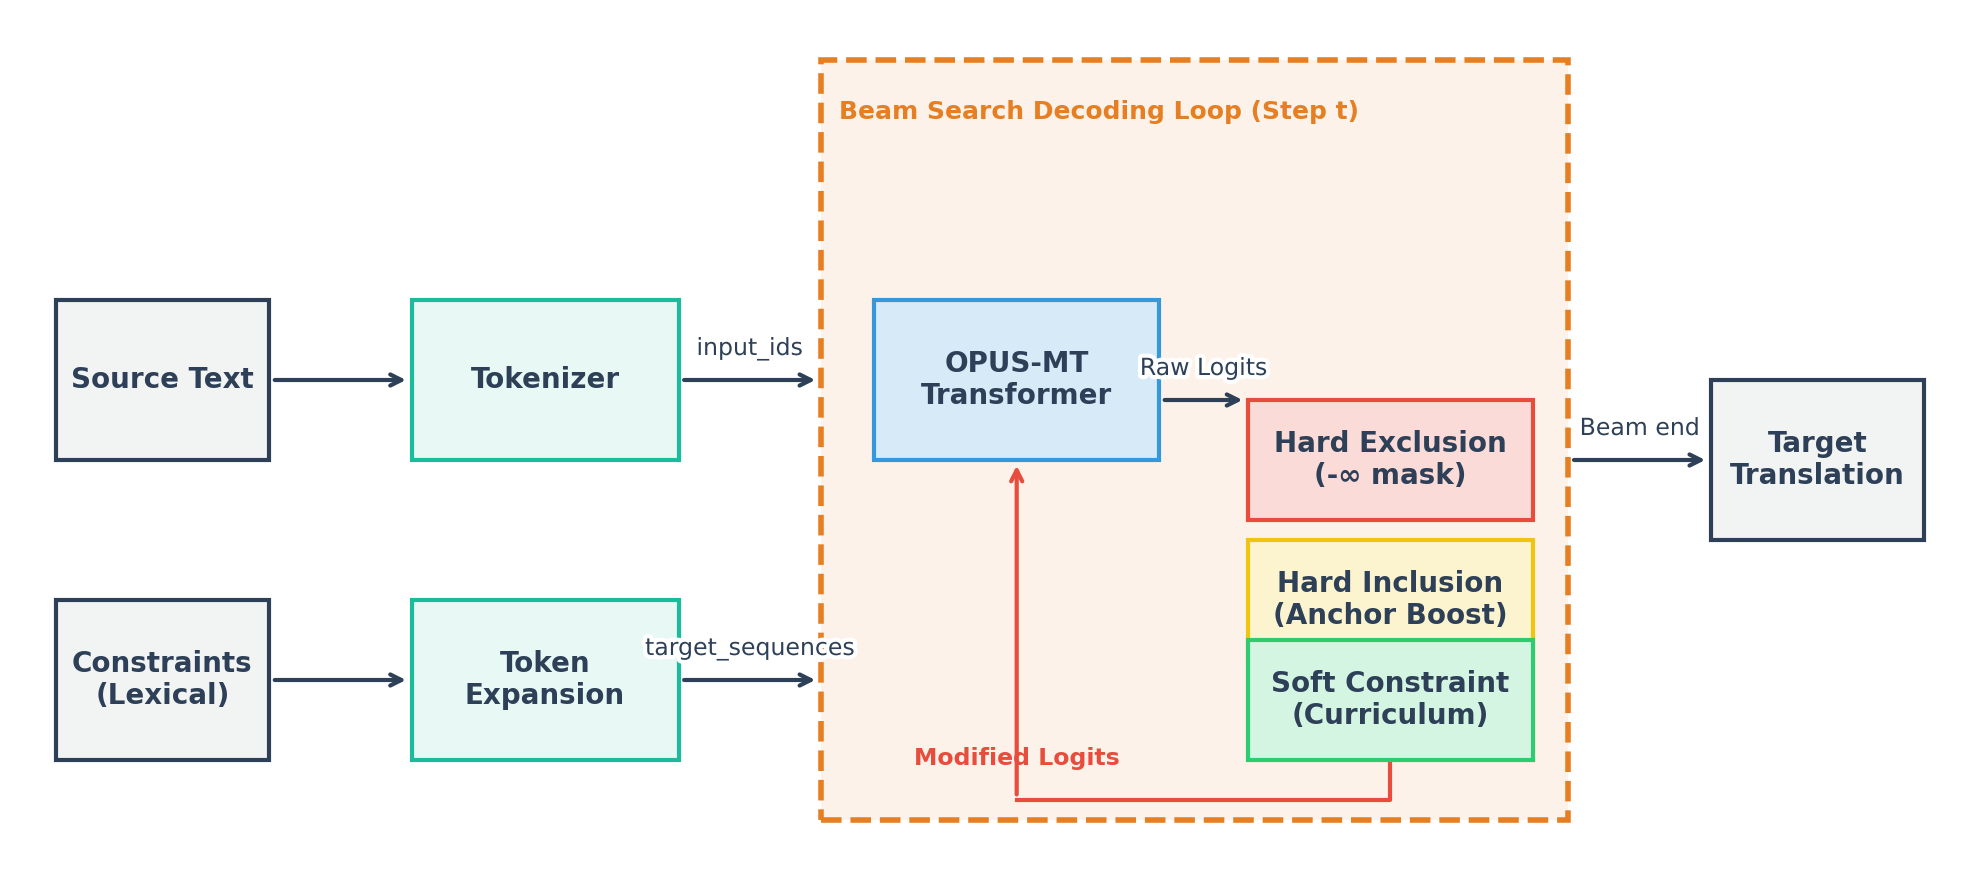
\includegraphics[width=0.8\textwidth]{fig0_architecture.png}
\caption{System architecture. At each decoding step, active LogitsProcessor instances inspect the partially generated token sequence and modify the raw output logits before beam selection.}
\label{fig:architecture}
\end{figure*}

\subsection{Hard Exclusion}

Hard exclusion prevents forbidden tokens from ever appearing in the output. At each step, the processor sets the logits of all forbidden token IDs to $-\infty$, effectively removing them from the distribution:
\begin{equation}
    l_t^{(i)} = -\infty \quad \forall\, i \in \mathcal{F},
\end{equation}
where $\mathcal{F}$ is the set of forbidden token IDs and $l_t^{(i)}$ is the logit for token $i$ at step $t$. This is a simple, zero-overhead operation that guarantees 100\% exclusion satisfaction without slowing down decoding.

\subsection{Hard Inclusion with Dynamic Anchor Scheduling}

Hard inclusion forces required words to appear in the output. The main challenge is that naively boosting a required token from step 1 disrupts sentence grammar: the model gets pushed toward a word before it has built up enough context for it to fit naturally.

Our processor addresses this with a \emph{dynamic anchor schedule}. For each pending required word, the processor computes how much logit pressure to apply based on three signals: (1) whether the current step is within an ``early token'' grace period $\tau$, (2) whether the required word's natural rank in the beam is already within an acceptable threshold $R_{\text{sweet}}$, and (3) the current sentence completion ratio $\rho = t / (0.8 \cdot L_{\text{src}})$, where $L_{\text{src}}$ is the source sentence length.

Formally, at step $t$, let $r_t$ be the natural rank of the required token $w$ in the current beam, and let $l_t^{(w)}$ be its logit. The applied boost $\delta_t$ is:
\begin{equation}
\resizebox{\columnwidth}{!}{$\displaystyle
\delta_t = \begin{cases}
    0 & \text{if } t \leq \tau \quad \text{(grace period)} \\
    \beta_{\text{sweet}} & \text{if } r_t \leq R_{\text{sweet}} \quad \text{(natural fit)} \\
    \max(0,\; l_t^{*} + A_{\text{start}} + A_{\text{range}} \cdot \rho - l_t^{(w)}) & \text{otherwise,}
\end{cases}
$}
\label{eq:anchor}
\end{equation}
where $l_t^{*}$ is the maximum logit across all tokens, $A_{\text{start}}$ and $A_{\text{range}}$ are the anchor offset and range hyperparameters, and $\beta_{\text{sweet}}$ is a small buffer applied when the word is already a high-probability candidate. The intuition is to delay aggressive intervention until the model has established enough syntactic context for the required word to fit naturally.

An EOS-blocking mechanism also prevents the model from ending the sentence while required words are still missing, unless the output has grown too long (beyond $1.5 \times L_{\text{src}}$ tokens), at which point a safety valve kicks in to stop runaway generation. Once a required multi-token sequence is placed, a morphological boundary penalty $\gamma_{\text{suffix}}$ is applied to discourage the model from immediately suffixing the constraint word with agglutinative morphemes.

\subsection{Soft Constraint Processor}

The soft constraint processor adjusts logits continuously without making any hard guarantees. It has two components that run together.

\emph{Soft Penalty.} For each penalty token $p \in \mathcal{P}$, the processor adds a fixed negative value $\lambda_{\text{pen}} < 0$:
\begin{equation}
    l_t^{(p)} \mathrel{+}= \lambda_{\text{pen}} \quad \forall\, p \in \mathcal{P}.
\end{equation}
This penalizes undesired words without strictly eliminating them.

\emph{Soft Curriculum Reward.} For pending reward tokens, the processor implements curriculum anchoring \cite{bengio2009curriculum}: the reward signal grows monotonically with the number of steps the reward has been active. Let $\eta$ be the number of active reward steps and $\lambda_{\text{rew}}$ be the base reward strength. The effective reward is:
\begin{equation}
    \lambda_{\text{eff}} = \min\!\left(\lambda_{\text{max}},\; \lambda_{\text{rew}} \cdot (1 + c \cdot \eta)\right),
\end{equation}
where $c$ is the curriculum growth rate and $\lambda_{\text{max}}$ caps the maximum pressure. To prevent early-token hallucination, reward application is suppressed for the first 3 decoding steps.

Rather than directly adding $\lambda_{\text{eff}}$ as a delta, the processor uses a \emph{target baseline} anchoring strategy: the reward token's logit is pulled up to $l_t^{*} + \theta_{\text{offset}} + \lambda_{\text{eff}}$ if it is below this baseline, or receives a small contextual nudge $\nu$ if it is already above it. This ensures that the required token remains competitive with the beam's top prediction without overwhelming the distribution.

\subsection{Combined Strategies}

\emph{Hard Combined.} The hard combined mode runs both exclusion and inclusion processors at the same time. Exclusion runs before inclusion so that the anchor calculation ignores masked tokens. If the order were reversed, the anchor could be calibrated against a forbidden token's high logit, over-boosting the required word.

\emph{Soft Combined.} The soft combined mode runs both penalty and reward components of SoftConstraintProcessor in a single pass, followed by a soft-boost retry pass if reward words are still missing after the first generation.

\subsection{Escalation Ladder (Soft Reward)}

The soft\_reward\_only function uses a three-tier escalation ladder: (1)~standard curriculum reward at the configured strength; (2)~maximum-strength soft boost targeting only the words still missing; (3)~hard inclusion as a last resort. The idea is to try the gentlest approach first and escalate only when needed. The downside is that difficult sentences may require up to three beam search passes.

\subsection{Hyperparameter Optimization}

We used Optuna \cite{akiba2019optuna} with the Tree-structured Parzen Estimator (TPE) sampler to find good parameter settings. Crucially, hyperparameters are optimized \emph{separately} for each translation direction on a dedicated HPO set, with the held-out evaluation set kept strictly separate.

For our proposed logit-level processors, we optimized a composite score that treats 1\% of constraint satisfaction as equivalent to 2 BLEU points:
\begin{equation}
    \text{score} = (S \times 200) + \overline{\text{BLEU}} - \mathcal{P}_{\text{len}},
    \label{eq:obj}
\end{equation}
where $S \in [0, 1]$ is the constraint satisfaction rate, $\overline{\text{BLEU}}$ is the mean BLEU score relative to the unconstrained baseline, and $\mathcal{P}_{\text{len}}$ is a quadratic length penalty:
\begin{equation}
    \mathcal{P}_{\text{len}} = \max(0,\; R_{\text{len}} - \theta)^2 \times 150{,}000,
    \label{eq:lenpen}
\end{equation}
with $\theta = 1.05$ for logit-level modes and $\theta = 1.03$ for DBA. $R_{\text{len}}$ is the average output-to-unconstrained length ratio. The quadratic form aggressively penalizes even moderate length inflation: a ratio of $1.10$ already contributes a penalty of $3{,}375$, fully eliminating candidates that pad outputs to satisfy constraints rather than placing them inline.

Trial budgets reflect the complexity of each search space: 50 trials for hard inclusion, hard combined, and soft combined (7 and 5 parameters with complex interactions); 30 trials for DBA (3 parameters); 10 trials for soft penalty (1 parameter with a flat landscape). The optimized hyperparameters for both directions are shown in Table~\ref{tab:hpo_params}.

\begin{table*}[!t]
\caption{Optimized Hyperparameters Found by Optuna TPE (50/10/30 trials per mode). All values are per-direction; EN→TR targets Turkish, TR→EN targets English. Parameters marked with $\dagger$ show the largest direction asymmetry.}
\label{tab:hpo_params}
\centering
\begin{tabular}{llrrp{5.8cm}}
\toprule
Group & Parameter & EN→TR & TR→EN & Role / Interpretation \\
\midrule
\multirow{7}{*}{\textbf{Hard Inclusion}}
  & Early-token grace $\tau$$^\dagger$ & 0 & 5
    & Steps before any boost is applied. Turkish targets benefit from immediate pressure ($\tau{=}0$); English targets improve with a short passive window. \\
  & Sweet-rank threshold $R_{\text{sweet}}$$^\dagger$ & 557 & 293
    & If the required word ranks below this in the beam, only a light buffer is applied instead of the full anchor boost. \\
  & Sweet-rank buffer $\beta_{\text{sweet}}$$^\dagger$ & 12.27 & 5.86
    & Logit boost applied when the word is already within the sweet-rank window (natural fit). \\
  & Anchor start $A_{\text{start}}$ & $-6.55$ & $-7.50$
    & Anchor target at 0\% sentence completion, expressed as offset below the current max logit. \\
  & Anchor range $A_{\text{range}}$ & 10.31 & 9.83
    & Total logit climb of the anchor target from 0\% to 100\% completion. \\
  & Inclusion boost & 5.74 & 7.18
    & Fixed logit boost applied when the required token is placed by the hard processor. \\
  & Suffix penalty $\gamma_{\text{suffix}}$$^\dagger$ & $-21.92$ & $-9.34$
    & Penalty applied immediately after a constraint word is placed to discourage agglutinative suffix attachment (stronger in Turkish targets). \\
\midrule
\multirow{4}{*}{\textbf{Soft Reward}}
  & Reward strength $\lambda_{\text{rew}}$ & 2.03 & 2.01
    & Base curriculum reward added to the required token's logit at each step. \\
  & Reward cap $\lambda_{\text{max}}$ & 15.37 & 19.04
    & Maximum reward that the curriculum schedule can reach. \\
  & Curriculum rate $c$ & 2.96 & 0.17
    & Controls how quickly the reward grows with active steps. \\
  & Anchor offset $\theta_{\text{offset}}$$^\dagger$ & $-23.89$ & $-28.74$
    & Reward baseline offset below the current max logit. Values $\lesssim{-}15$ create a passive safety net; values near 0 force early injection and hurt BLEU. \\
\midrule
\multirow{1}{*}{\textbf{Soft Penalty}}
  & Penalty $\lambda_{\text{pen}}$ & $-98.37$ & $-118.52$
    & Any value $\lesssim{-}30$ produces identical results (threshold suppression); exact magnitude is not critical. \\
\midrule
\multirow{3}{*}{\textbf{DBA Baseline}}
  & Beam size$^\dagger$ & 7 & 5
    & More beams needed in EN→TR for the allocator to encounter Turkish surface forms. \\
  & Length penalty$^\dagger$ & $+0.01$ & $-4.61$
    & Near-zero in EN→TR (length cannot be controlled); strongly negative in TR→EN to curb residual appending. \\
  & Repetition penalty & 1.03 & 1.20
    & Discourages DBA's tendency to repeat tokens or punctuation in appended suffixes. \\
\bottomrule
\end{tabular}
\end{table*}


% =============================================================================
\section{Experimental Setup}
% =============================================================================

\subsection{Models and Hardware}

All experiments use the Helsinki-NLP OPUS-MT ``big'' transformer models: opus-mt-tc-big-en-tr for English-to-Turkish and opus-mt-tc-big-tr-en for Turkish-to-English \cite{tiedemann2020opus, tiedemann2023democratizing}. These are 6-layer encoder-decoder transformers with 8 attention heads and a model dimension of 512. Models are downloaded and cached locally. We ran everything on a single NVIDIA GPU with CUDA support, using PyTorch \cite{paszke2019pytorch} in no-gradient inference mode.

\subsection{Test Set}

We built a bilingual evaluation set of 500 sentence pairs (250 EN→TR, 250 TR→EN) derived from the Tatoeba English--Turkish test split \cite{tiedemann2020tatoeba}. Constraints are generated automatically by comparing each human reference against the unconstrained OPUS-MT baseline: words present in the reference but missing from the baseline become \emph{required} constraints, and vice versa for \emph{forbidden} constraints. We check morphological overlap to avoid penalizing relatives of required words. Cases are split evenly between \emph{easy} (baseline nearly produces the word) and \emph{hard} (baseline omits it entirely) instances, then divided into dedicated HPO and held-out evaluation sets.

Each case specifies forbidden/required words for hard modes, and corresponding penalty/reward words for soft modes. The baseline translation is computed once per sentence. Exclusion-only modes are evaluated on the 163 EN→TR and 142 TR→EN cases with exclusion annotations; inclusion-bearing and combined modes use the 250 EN→TR and 247 TR→EN cases with required-word annotations.

\subsection{Evaluation Metrics}

We measure each mode on four fronts. \emph{Constraint Satisfaction Rate} ($S$): the fraction of test cases where all required words appear in the output (inclusion) and no forbidden words appear (exclusion), checked with a morphology-aware matcher that accepts valid Turkish inflectional suffixes. \emph{Baseline BLEU}: computed against the unconstrained baseline output, so it captures how much the constraint changes the output rather than absolute quality---a Baseline BLEU of 100 means the constraint had no effect. \emph{Reference BLEU} \cite{papineni2002bleu} and \emph{ChrF} \cite{popovic2015chrf}: both computed against human ground-truth reference translations, measuring absolute translation quality. \emph{Length Ratio}: average constrained-to-unconstrained output length, which serves as a quick diagnostic for word-appending artifacts.

\subsection{Evaluation Protocol}

All reported results are averaged over three random seeds (42, 123, 7) to reduce stochastic noise in the pipeline. For the DBA baseline, we use HuggingFace's \texttt{DisjunctiveConstraint} to encompass all suffix and capitalization variants for required words, and provide a complete \texttt{flat\_token\_ids} map for \texttt{bad\_words\_ids}---a maximally generous configuration.

% =============================================================================
\section{Results and Discussion}
% =============================================================================

\subsection{Aggregate Results}

Tables~\ref{tab:results_en_tr} and~\ref{tab:results_tr_en} summarize the aggregate metrics for EN→TR and TR→EN respectively, averaged over three seeds. We report Baseline BLEU, Reference BLEU, ChrF, decoding latency, and the average number of generation passes. The hard\_inclusion\_ablation mode (identical code path to hard\_inclusion, included as a pipeline sanity check) confirmed matching results and is omitted here for brevity.

\subsection{Hard Constraint and DBA Baseline Analysis}

Hard exclusion achieves 98.2\% satisfaction in EN→TR and 99.3\% in TR→EN, with very low length inflation in both directions (ratios of 1.009 and 1.016). The model rephrases to avoid forbidden terms without significant elongation.

Hard inclusion achieves 99.6\%/99.2\% satisfaction in EN→TR/TR→EN---both improvements over the previous single-direction figure of 97.6\%. Baseline BLEU scores show direction asymmetry: 50.49 in EN→TR versus 73.93 in TR→EN. This gap reflects the fundamentally harder constraint problem in agglutinative Turkish targets, where the model must place a required word while also managing suffix attachment and morphophonological agreement, leaving less room for natural phrasing.

The HuggingFace DBA baseline reveals a critical direction-dependent failure. In EN→TR, DBA reaches only a 2.768 average length ratio, meaning outputs are nearly \emph{three times} the expected length. The structural beam allocator, unable to find valid Turkish surface forms among its beam hypotheses, resorts to appending constraint words at the end of otherwise complete translations, often entering repetitive punctuation loops. Qualitative inspection of EN→TR DBA outputs confirms strings such as \emph{``\dots değil mi?.. b\dots???!??.\,? ???\dots??''} appended after legitimate translations. The Baseline BLEU of 31.17 for EN→TR DBA is therefore a consequence of this length explosion rather than a direct quality failure---the underlying translation up to the appended portion is often reasonable.

In TR→EN, the picture is considerably better: DBA achieves a 1.289 length ratio and 97.2\% satisfaction. English targets, being morphologically simple, allow DBA to find constraint words within the natural beam hypotheses without resorting to appending. This direction-asymmetric behavior limits DBA's practical applicability for EN→TR in our setting.

In contrast, our hard inclusion maintains a 1.063/1.062 length ratio in both directions and runs 2.1$\times$ faster than DBA in EN→TR (943.3 vs.\, 2003.3~ms) and 3.3$\times$ faster in TR→EN (239.9 vs.\, 784.0~ms). Fig.~\ref{fig:length_ratio} and Fig.~\ref{fig:latency} make these comparisons explicit.

\subsection{Combined and Soft Constraint Analysis}

Hard combined enforces exclusion and inclusion simultaneously, but shows non-linear degradation (the \emph{logit squeeze effect}) below what either isolated mode achieves: EN→TR reaches 91.2\% satisfaction with 32.53 Baseline BLEU, while TR→EN reaches 96.0\% satisfaction with 56.55 Baseline BLEU. This asymmetry appears to stem from the fact that Turkish exclusion masks more token IDs per forbidden word (since agglutinative morphology generates more surface variants), narrowing the beam distribution aggressively and leaving less room for the inclusion anchor to operate.

For soft constraints, soft penalty produces results that are numerically identical to hard exclusion: the same satisfaction rates, BLEU scores, and length ratios. This stems from \emph{threshold suppression} in beam search, where penalties sufficiently negative to push a forbidden token out of the top-$K$ beam effectively mimic a hard $-\infty$ mask. Under our configuration, soft penalty offered no measurable advantage over hard exclusion. Soft reward with escalation achieves the best overall trade-off: 99.2\%/98.8\% satisfaction and 72.32/81.65 Baseline BLEU, with the escalation ladder activating on roughly 40\% of sentences. Soft combined drops satisfaction to 62.0\%/71.3\% due to competing penalty and reward forces.

Fig.~\ref{fig:quality_overview} shows the full quality breakdown across all modes for both directions.

\subsection{Dynamic Scheduling and Hyperparameter Sensitivity}

Fig.~\ref{fig:anchor_heatmap} shows the dynamic anchoring schedule simulated using the optimized parameters. The EN→TR schedule applies immediate pressure ($\tau = 0$) starting at $A_{\text{start}} = -6.55$ and climbing by $A_{\text{range}} = 10.31$. Conversely, TR→EN uses $\tau = 5$ grace steps, $A_{\text{start}} = -7.50$, and $A_{\text{range}} = 9.83$. This difference suggests that English targets benefit from immediate constraint pressure, whereas Turkish targets require a short passive window to establish syntactic structure.

Hyperparameter optimization (HPO) studies reveal distinct structural sensitivities. Soft penalty is one-shot: any value more negative than roughly $-30$ pushes tokens outside the top-$K$ beam, making search optimization unnecessary. Soft reward, conversely, exhibits a large flat optimum. Because the reward baseline only intervenes when the required word's probability drops below a safe threshold, offsets $\lesssim -15$ act as a passive safety net. Once this anchor becomes sufficiently passive, exact parameter values matter very little; the model maintains its natural fluency and only receives a targeted boost when it genuinely threatens to omit the constraint word. Hard inclusion displays a much more highly sensitive landscape across its seven parameters. Because it must forcefully inject tokens while simultaneously calculating anchor climbs and suffix penalties, it requires the full 50-trial budget to carefully calibrate these cooperating settings. DBA tuning is similarly asymmetric, converging to 7 beams with near-zero length penalty in EN$\rightarrow$TR to force Turkish surface forms into the beam, and 5 beams with negative penalty in TR$\rightarrow$EN to check length inflation.

\clearpage

\begin{table*}[!t]
\caption{Aggregate Results — English to Turkish (EN→TR, $N_{\text{excl}}=163$, $N_{\text{incl}}=250$)}
\label{tab:results_en_tr}
\centering
\begin{tabular}{lcccccccc}
\toprule
Mode & $N$ & Sat.\,\% & BLEU (Base) & BLEU (Ref) & ChrF (Ref) & Len. Ratio & Latency (ms) & Passes \\
\midrule
Unconstrained           & 250 & --     & 100.00 & 40.97 & 67.04 & 1.000 & \phantom{0}96.9 & 1.00 \\
\midrule
Hard Exclusion          & 163 & 98.2\% & \phantom{0}35.20 & 35.59 & 58.84 & 1.009 & 165.2  & 1.00 \\
Hard Inclusion          & 250 & 99.6\% & \phantom{0}50.49 & 31.11 & 65.88 & 1.063 & 943.3  & 1.00 \\
Hard Combined           & 250 & 91.2\% & \phantom{0}32.53 & 34.98 & 65.04 & 1.114 & 1082.6 & 1.00 \\
\midrule
Soft Penalty            & 163 & 98.2\% & \phantom{0}35.20 & 35.59 & 58.84 & 1.009 & 167.9  & 1.00 \\
Soft Reward (Escal.)    & 250 & 99.2\% & \phantom{0}72.32 & 40.98 & 71.31 & 1.062 & 838.0  & 1.79 \\
Soft Combined           & 250 & 62.0\% & \phantom{0}57.65 & 47.62 & 68.53 & 1.007 & 386.6  & 1.37 \\
\midrule
HuggingFace DBA         & 250 & 97.6\% & \phantom{0}31.17 & 34.41 & 62.39 & 2.768  & 2003.3 & 1.00 \\
\bottomrule
\end{tabular}
\end{table*}

\begin{table*}[!t]
\caption{Aggregate Results — Turkish to English (TR→EN, $N_{\text{excl}}=142$, $N_{\text{incl}}=247$)}
\label{tab:results_tr_en}
\centering
\begin{tabular}{lcccccccc}
\toprule
Mode & $N$ & Sat.\,\% & BLEU (Base) & BLEU (Ref) & ChrF (Ref) & Len. Ratio & Latency (ms) & Passes \\
\midrule
Unconstrained           & 250 & --     & 100.00 & 49.55 & 66.99 & 1.000 & 101.2 & 1.00 \\
\midrule
Hard Exclusion          & 142 & 99.3\% & \phantom{0}44.74 & 40.58 & 61.52 & 1.016 & 188.4 & 1.00 \\
Hard Inclusion          & 247 & 99.2\% & \phantom{0}73.93 & 44.86 & 69.57 & 1.062 & 239.9 & 1.00 \\
Hard Combined           & 247 & 96.0\% & \phantom{0}56.55 & 51.07 & 72.66 & 1.050 & 399.4 & 1.00 \\
\midrule
Soft Penalty            & 142 & 99.3\% & \phantom{0}44.74 & 40.58 & 61.52 & 1.016 & 184.6 & 1.00 \\
Soft Reward (Escal.)    & 247 & 98.8\% & \phantom{0}81.65 & 49.07 & 71.65 & 1.058 & 314.5 & 1.71 \\
Soft Combined           & 247 & 71.3\% & \phantom{0}66.52 & 54.75 & 71.62 & 1.013 & 236.8 & 1.32 \\
\midrule
HuggingFace DBA         & 250 & 97.2\% & \phantom{0}49.08 & 50.38 & 70.36 & 1.289  & 784.0 & 1.00 \\
\bottomrule
\end{tabular}
\end{table*}

\begin{figure*}[!t]
\centering
\begin{minipage}{0.75\textwidth}
  \centering
  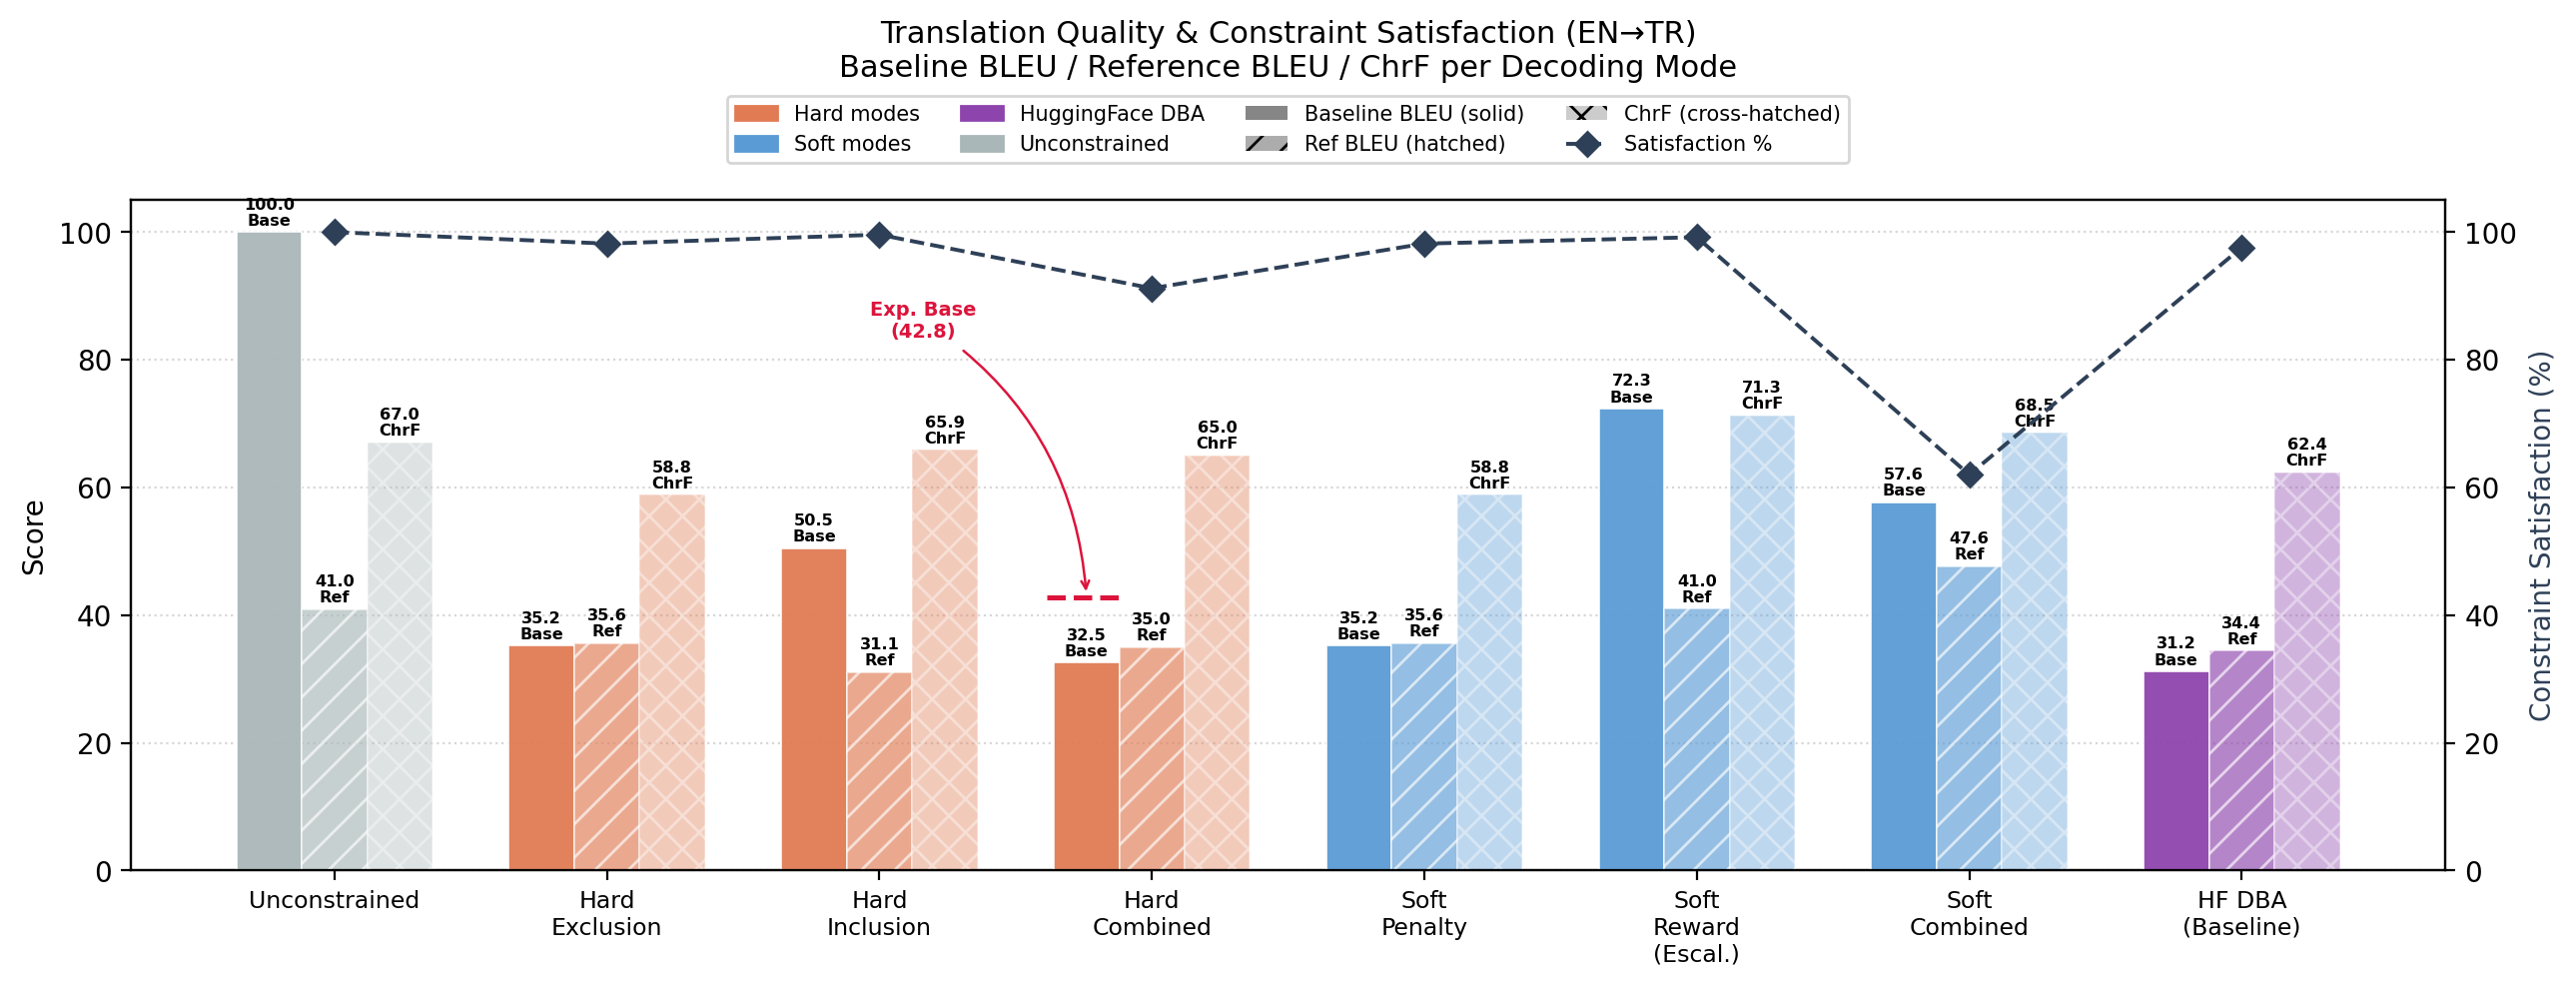
\includegraphics[width=\textwidth]{fig1_quality_overview_en_tr.png}
  \centerline{\small (a) EN→TR}
\end{minipage}
\par\vspace{0.2cm}
\begin{minipage}{0.75\textwidth}
  \centering
  
\includegraphics[width=\textwidth]{fig1_quality_overview_tr_en.png}
  \centerline{\small (b) TR→EN}
\end{minipage}
\caption{Translation quality (Baseline BLEU / Reference BLEU / ChrF) and constraint satisfaction per decoding mode, for both translation directions.}
\label{fig:quality_overview}
\end{figure*}

\setcounter{dbltopnumber}{4}
\renewcommand{\dbltopfraction}{0.99}
\renewcommand{\textfraction}{0.01}
\renewcommand{\dblfloatpagefraction}{0.99}

\begin{figure*}[!t]
\centering
\begin{minipage}{0.6\textwidth}
  \centering
  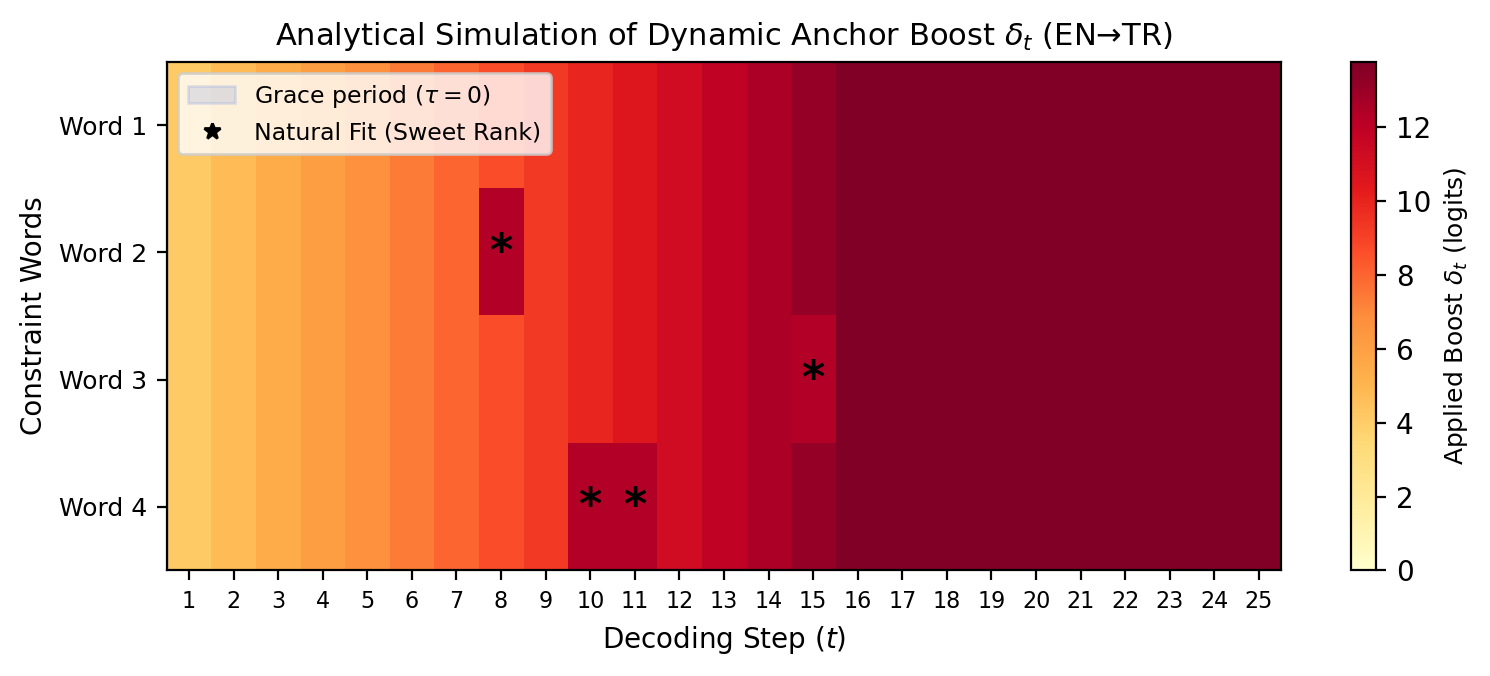
\includegraphics[width=\textwidth]{fig3_anchor_heatmap_en_tr.png}
  \centerline{\small (a) EN→TR ($\tau=0$, $A_\text{start}=-6.55$, $A_\text{range}=10.31$)}
\end{minipage}
\par\vspace{0.1cm}
\begin{minipage}{0.6\textwidth}
  \centering
  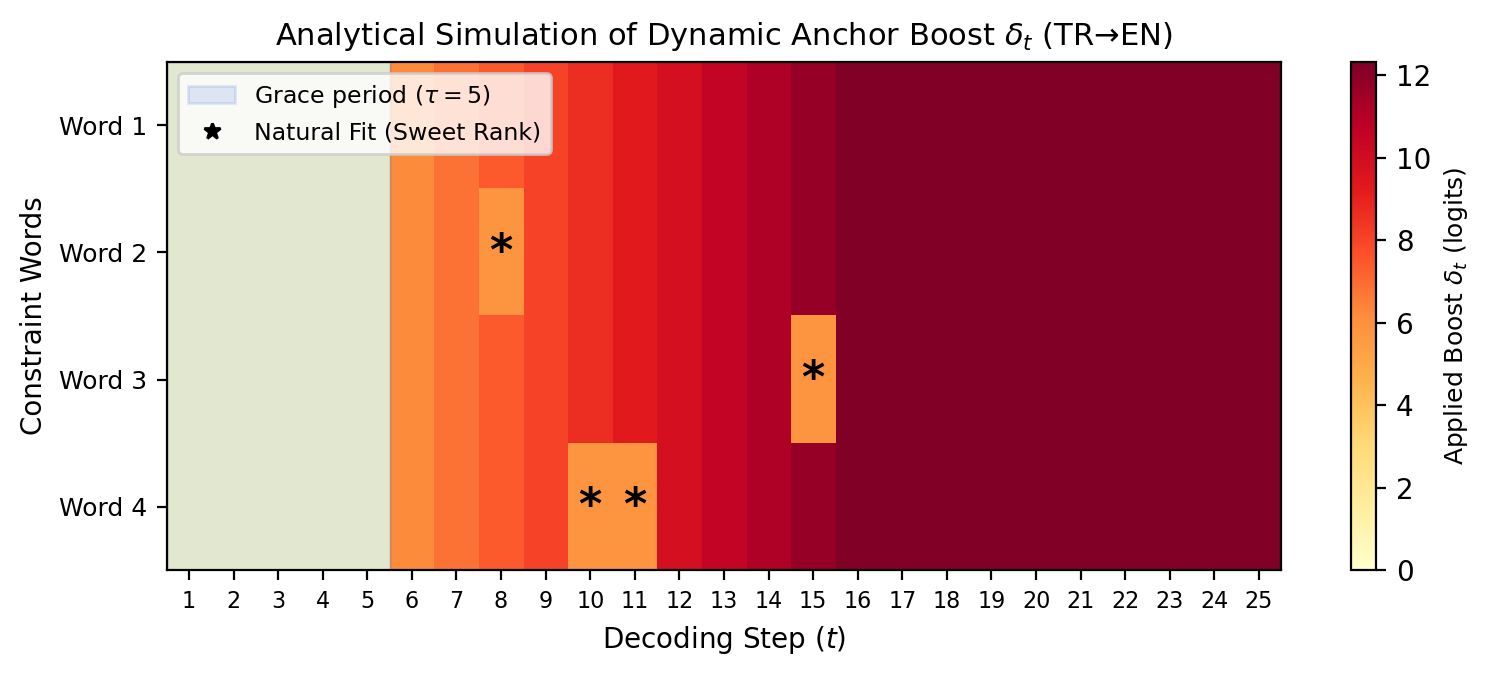
\includegraphics[width=\textwidth]{fig3_anchor_heatmap_tr_en.png}
  \centerline{\small (b) TR→EN ($\tau=5$, $A_\text{start}=-7.50$, $A_\text{range}=9.83$)}
\end{minipage}
\caption{Dynamic anchor schedule for each direction. Color intensity indicates applied logit boost $\delta_t$. The grace period (zero boost), sweet-rank windows (light buffer), and full anchor pressure are distinguishable. The EN→TR direction applies pressure from step~1; TR→EN waits five steps.}
\label{fig:anchor_heatmap}
\end{figure*}

\begin{figure*}[!t]
\centering
\begin{minipage}{0.6\textwidth}
  \centering
  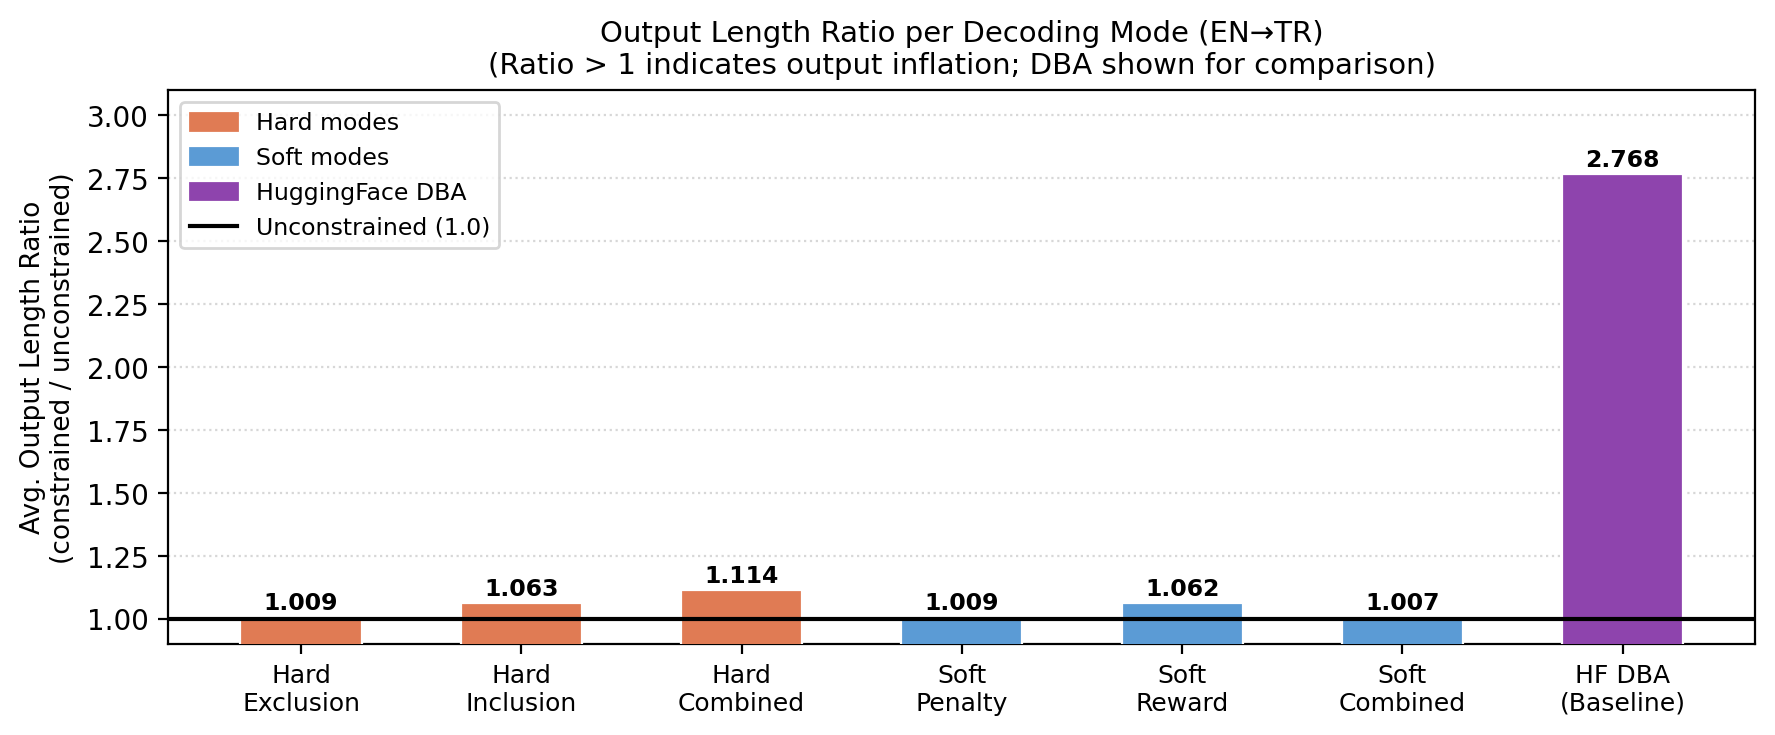
\includegraphics[width=\textwidth]{fig4_length_ratio_en_tr.png}
  \centerline{\small (a) EN→TR}
\end{minipage}
\par\vspace{0.1cm}
\begin{minipage}{0.6\textwidth}
  \centering
  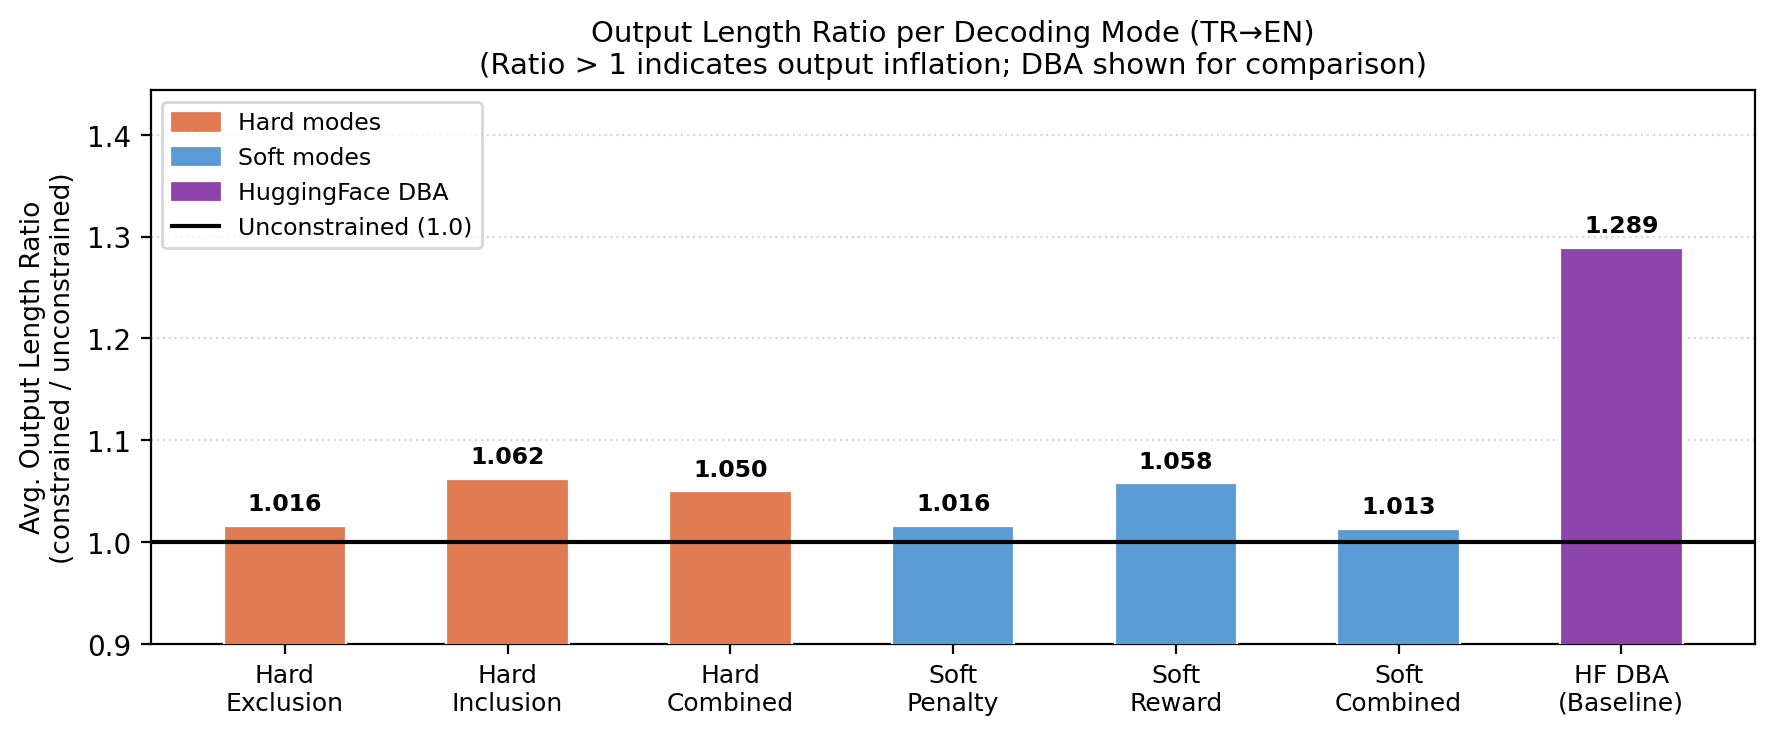
\includegraphics[width=\textwidth]{fig4_length_ratio_tr_en.png}
  \centerline{\small (b) TR→EN}
\end{minipage}
\caption{Output length ratio per decoding mode. DBA's length inflation is severe in EN→TR (2.768) due to agglutinative Turkish morphology, and moderate in TR→EN (1.289). All logit-level modes remain below 1.12 in both directions.}
\label{fig:length_ratio}
\end{figure*}

\clearpage

\twocolumn[{%
  \begin{center}
    \begin{minipage}{0.75\textwidth}
      \centering
      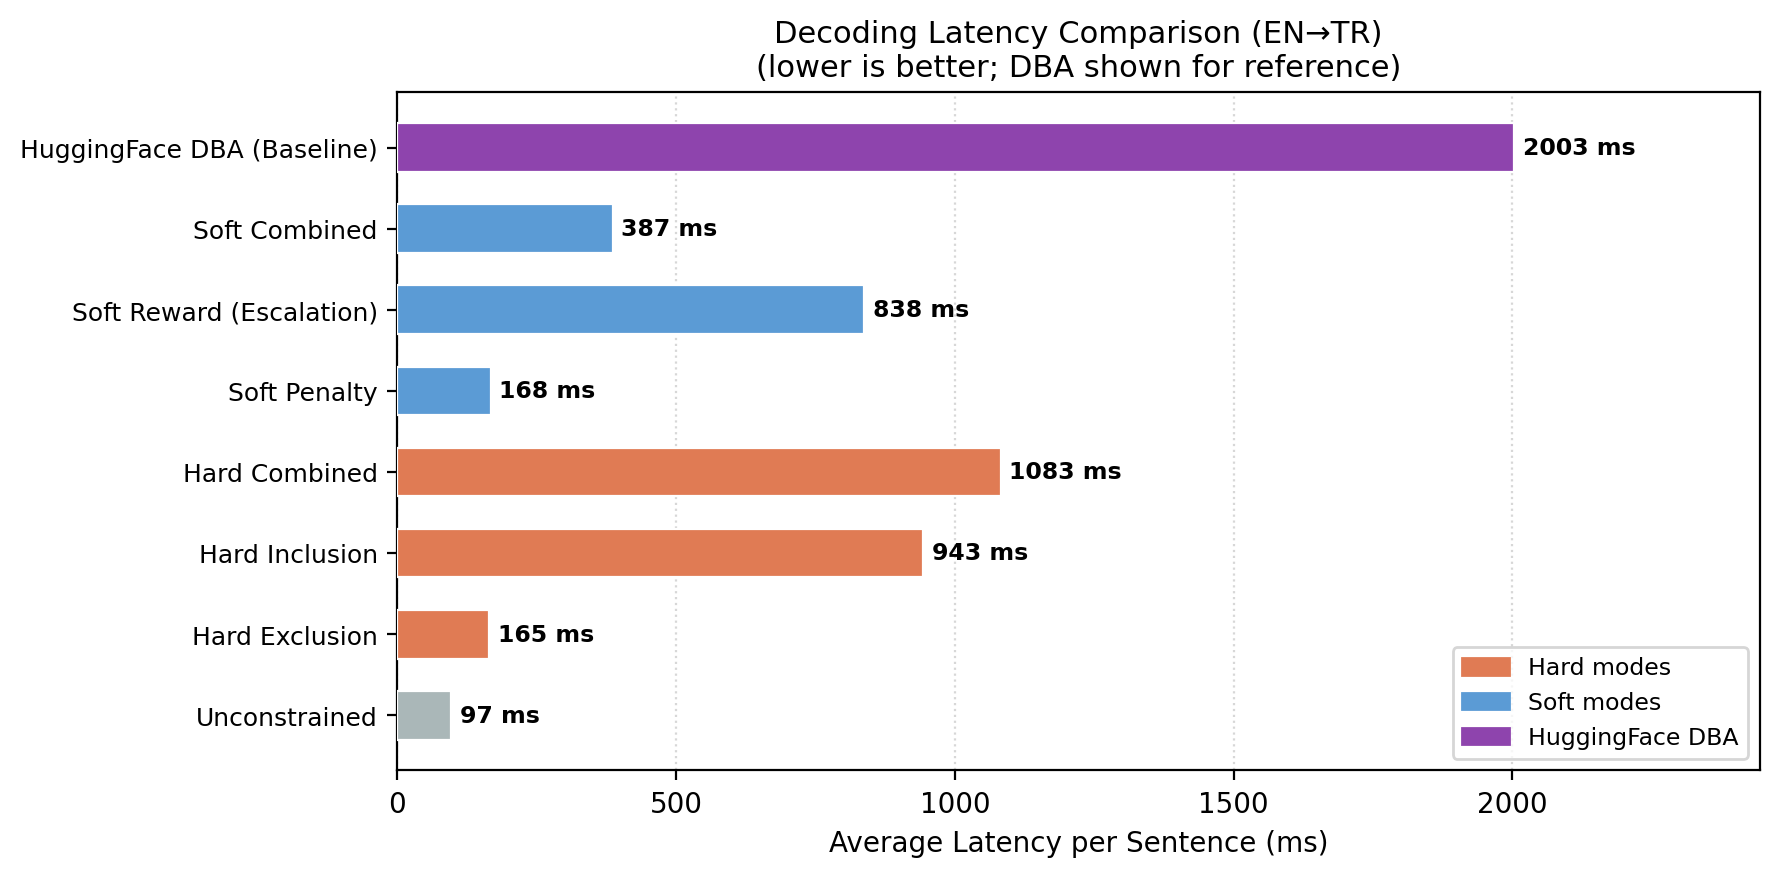
\includegraphics[width=\textwidth]{fig6_latency_en_tr.png}
      \centerline{\small (a) EN→TR}
    \end{minipage}
    \par\vspace{0.2cm}
    \begin{minipage}{0.75\textwidth}
      \centering
      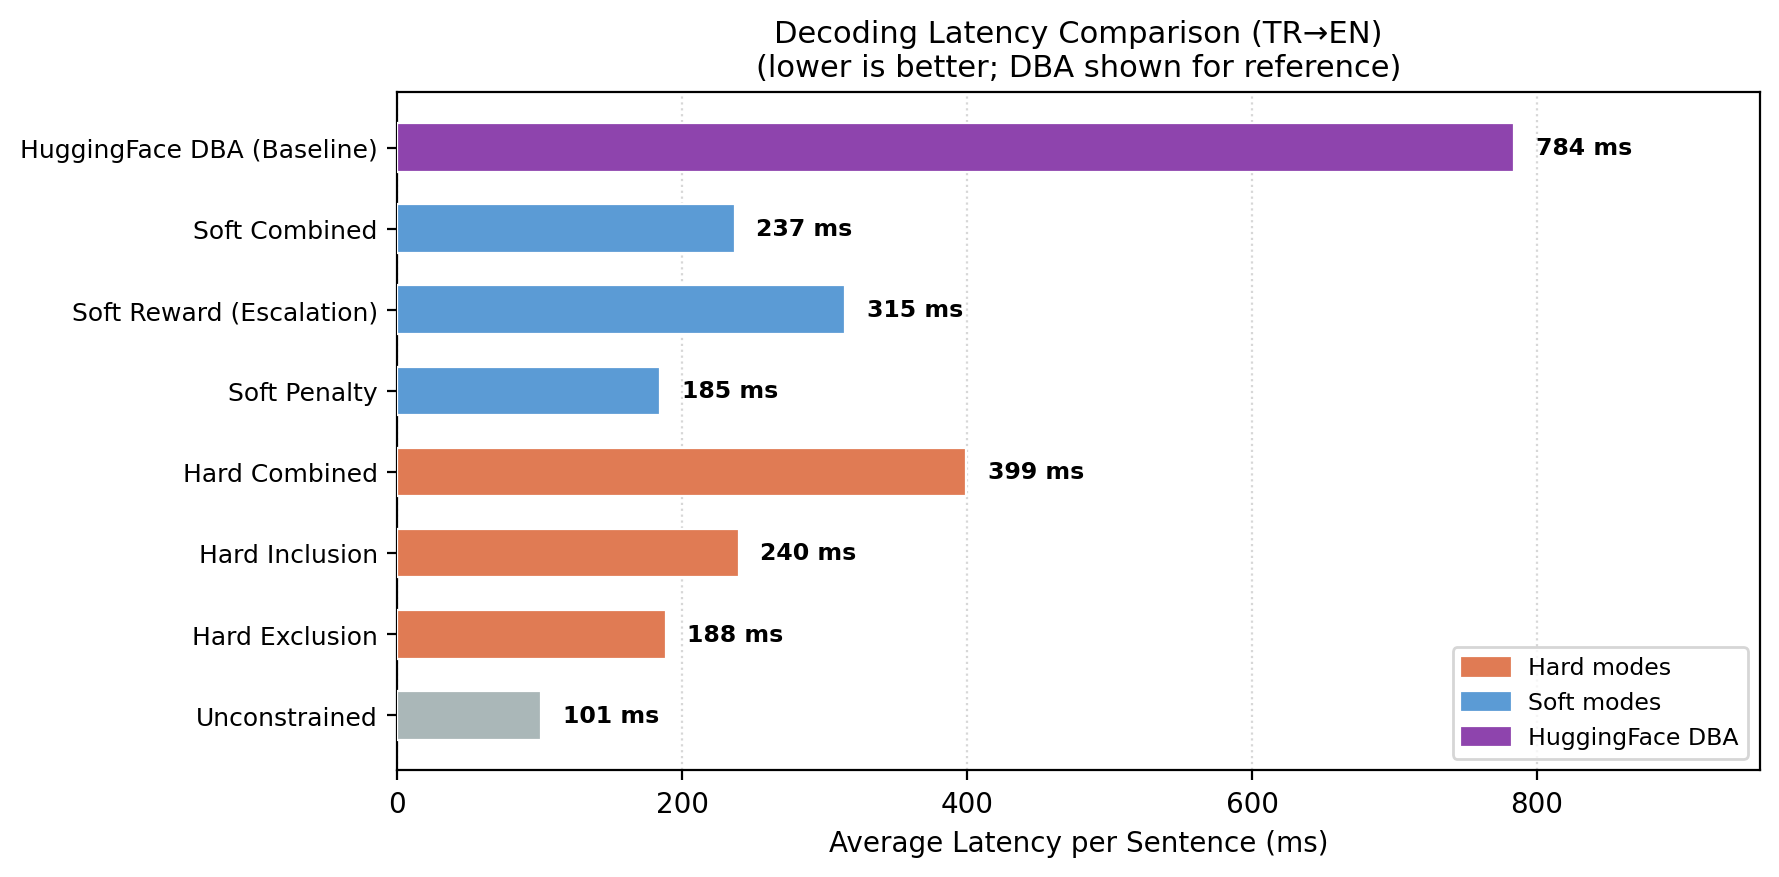
\includegraphics[width=\textwidth]{fig6_latency_tr_en.png}
      \centerline{\small (b) TR→EN}
    \end{minipage}
    \vspace{0.3cm}
    
    \begin{minipage}{0.95\textwidth}
      \refstepcounter{figure}\label{fig:latency}
      \small \textbf{Fig. \thefigure.} Average decoding latency per sentence for all modes and the DBA baseline. Logit-level methods run well under 1000~ms; DBA requires over 2000~ms in EN→TR and 784~ms in TR→EN.
    \end{minipage}
    \vspace{0.6cm}
  \end{center}
}]

\subsection{Qualitative and Morphological Analysis}

Qualitative inspection of hard inclusion failures highlights three limitations: (1) competing schedules for multiple constraints resulting in repetition (e.g., repeating \emph{uzay istasyonu} instead of producing both \emph{uzay istasyonu} and \emph{yörünge}); (2) semantic mismatch where syntax templates lock in baseline synonyms (e.g., \emph{movies} instead of \emph{cinema}); and (3) ungrammatical insertion from simultaneous logit pressure (e.g., \emph{The little dog tiny barked}).

Furthermore, word-appending artifacts in Turkish stem from the agglutination mismatch. When the constraint is a bare root (e.g., \emph{hekim}) but the model prefers an inflected form (e.g., \emph{hekimin}), exact-match checks fail, and EOS-blocking appends the bare root at the end. Suffix expansion and suffix penalties address this, yielding a 99.6\% EN→TR satisfaction rate, but complex suffix chains remain difficult to cover fully.

\subsection{Methodological Transparency}

We note three main limitations. First, while the corpus is split into HPO and evaluation sets, both are drawn from the same curated bilingual source, so some distributional overlap remains. Second, the soft reward mode's strong results require up to three beam search passes per sentence, which may not be practical for latency-sensitive applications. Third, Reference BLEU and ChrF are computed against a single human reference per sentence and may not fully reflect output quality for sentences with many equally valid translations.

\subsection{Conclusion}
% =============================================================================

Across both translation directions, curriculum-based soft reward provides the best balance between lexical satisfaction and translation quality, while hard inclusion offers a faster alternative to DBA without its severe length inflation in English→Turkish. These results suggest that logit-level control can compete with structural constrained decoding while requiring far fewer modifications to existing decoding pipelines. Future research will explore joint training of constraint processors and morphology-aware constraint metrics specifically tailored for agglutinative target languages.

\bibliographystyle{IEEEtran}
\bibliography{references}

\end{document}